\chapter{Исследовательская часть}
В этом разделе будут проведены исследования полученных результатов.
\section{Технические характеристики}
Технические характеристики устройства, на котором выполнялось тестирование, следующие:
\begin{itemize}
	\item операционная система: Ubuntu 20.04.1 LTS; \cite{ubuntu}
	\item память: 8 GB;
	\item процессор: Intel Core i5-1135G7 @ 2.40GHz \cite{intel}.
	\item количество ядер процессора: 8
\end{itemize}

Во время тестирования ноутбук был нагружен только встроенными приложениями окружения, а также непосредственно системой тестирования.

\section{Метод тестирования}
Для проведения замеров времени в экспериментах будет использована формула 4.1:
\begin{equation}
t = \frac{T_n}{N}
\end{equation}
где $t$ -- время выполнения реализации алгоритма, $N$ - количество экспериментов, $T_n$ - время выполнения замеров.

Неоднократное измерение времени необходимо для построения более гладкого графика и получения усреднённого значения.
Для замеры общего времени используется библиотека chrono.

\section{Демонстрация работы программы}
На рисунке 4.1 представлена демонстрация работы программы:
\FloatBarrier
\begin{figure}[h]
	\begin{center}
		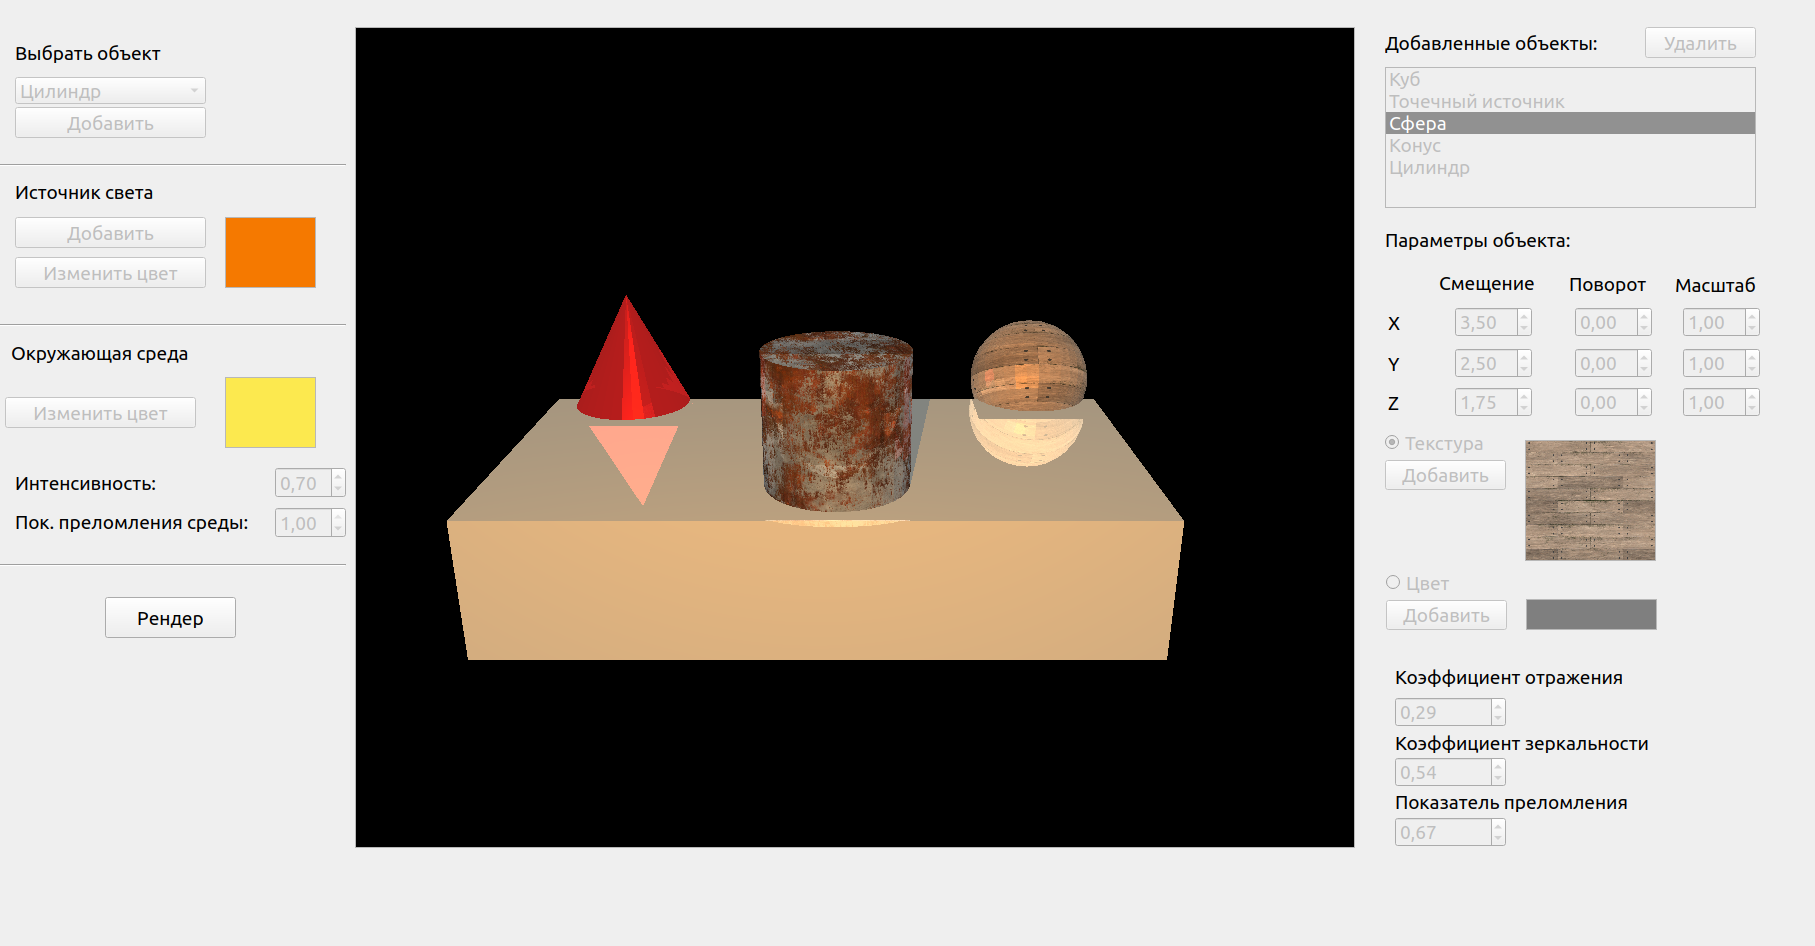
\includegraphics[width=\linewidth]{inc/demonstrate.png}
	\end{center}
	\caption{Демонстрация работы программы}
\end{figure}
\FloatBarrier

\section{Зависимость времени работы алгоритма обратной трассировки лучей от количества объектов в сцене}
Время работы алгоритма обратной трассировки лучей имеет зависимость от количества объектов в сцене.
Для измерения времени работы алгоритма на сцены добавлялось $ N $ сфер, для которых и подсчитывалось время работы.
Также на сцене находится один точечный источник. 

Тестирование производилось на следующих параметрах:
\begin{enumerate}
	\item Количество потоков -- 8.
	\item Глубина рекурсии -- 2.
	\item Интенсивность окружающего света -- 0.5.
	\item Коэффициент преломления внешней среды -- 1.
	\item Коэффициент отражения объекта -- 0.2.
	\item Коэффициент преломления объекта -- 0.5.
\end{enumerate}

Тестирование также проводилось для двух случаев:
\begin{enumerate}
	\item Сфера закрашивается цветом.
	\item Сфера имеет текстуру.
\end{enumerate}

В таблице 4.1 приведены результаты тестирования работы алгоритмов в случае закраски цветом:
\FloatBarrier
\begin{table}[h]
	\caption{Результаты тестов}
	\centering
	\begin{tabular}{ | c | c |}
		\hline
		Количество объектов & Время (в мс) \\ 
		\hline
		1 & 12160274 \\
		2 & 25475533 \\
		3 & 42793308 \\
		4 & 62433652 \\
		\hline
	\end{tabular}
\end{table}
\FloatBarrier

В таблице 4.2 приведены результаты тестирования работы алгоритмов в случае текстуризации:
\FloatBarrier
\begin{table}[h]
	\caption{Результаты тестов}
	\centering
	\begin{tabular}{ | c | c |}
		\hline
		Количество объектов & Время (в мс) \\ 
		\hline
		1 & 13439190 \\
		2 & 22993890 \\
		3 & 49343762 \\
		4 & 89433652 \\
		\hline
	\end{tabular}
\end{table}
\FloatBarrier

На рисунке 4.2 представлены графики зависимости времени работы алгоритма от количества объектов в сцене
\FloatBarrier
\begin{figure}[h]
	\begin{center}
		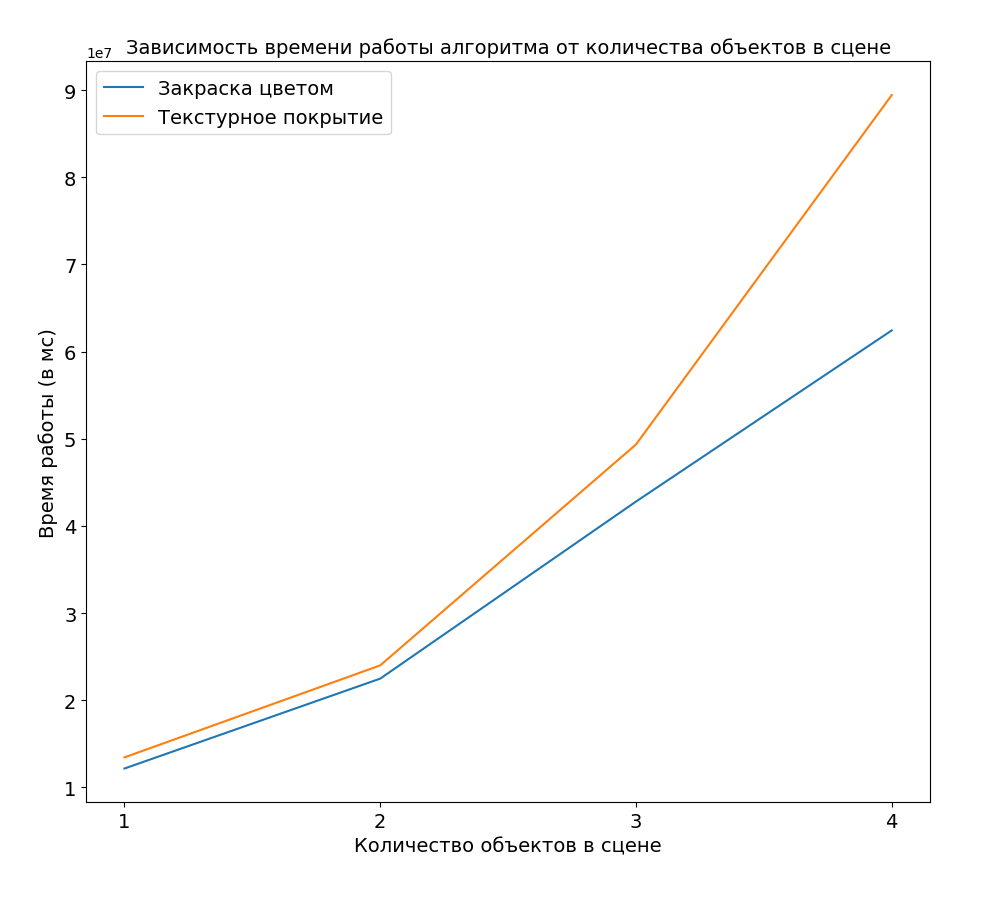
\includegraphics[width=\linewidth]{inc/obj.png}
	\end{center}
	\caption{График зависимости времени работы алгоритма от количества объектов в сцене}
\end{figure}
\FloatBarrier

\section{Зависимость времени работы алгоритма обратной трассировки лучей от количества потоков программы}
Особенностью алгоритма обратной трассировки лучей является то, что каждый луч работает независимо друг от друга.
Следовательно, вычисления могут производиться параллельно.
В программе это реализовано следующим образом: картинка делилась на $n$ частей по диагонали, а затем каждый из $n$ потоков работал на своей части.

В качестве сцены для тестирования использовалась следующая композиция объектов: сфера, цилиндр, конус, куб и точечный источник света.
У всех объектов одинаковые параметры:

В таблице 4.3 приведены результаты тестирования работы алгоритма от количества потоков:
\FloatBarrier
\begin{table}[h]
	\caption{Результаты тестов}
	\centering
	\begin{tabular}{ | c | c |}
		\hline
		Количество объектов & Время (в мс) \\ 
		\hline
		1 & 38771415 \\
		2 & 27341234 \\
		4 & 18204997 \\
		8 & 16129667 \\
		16 & 20010097\\
		\hline
	\end{tabular}
\end{table}
\FloatBarrier

На рисунке 4.3 представлен график зависимости времени работы алгоритма от количества потоков:
\FloatBarrier
\begin{figure}[h]
	\begin{center}
		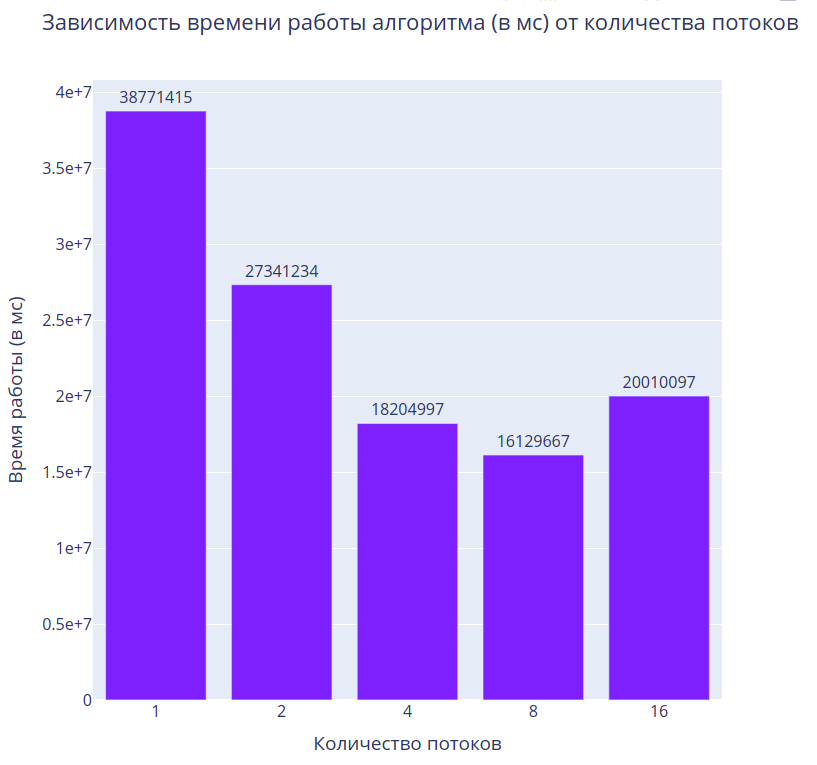
\includegraphics[height = 12cm, width=14cm]{inc/thread.png}
	\end{center}
	\caption{График зависимости времени работы алгоритма от количества потоков}
\end{figure}
\FloatBarrier

\section{Зависимость времени работы алгоритма обратной трассировки лучей от глубины рекурсии}
В алгоритме обратной трассировки лучей для каждого луча проверяется, достигнута ли глубина рекурсии.
В случае, если не достигнута, рассчитывается направление и интенсивность отражённого и преломлённого лучей.

Чем меньше глубина рекурсии, тем меньше время работы программы, но полученное изображение менее реалистическое.
В качестве сцены для тестирования использовалась следующая композиция объектов: сфера, цилиндр, конус, куб и точечный источник света.

В таблице 4.4 приведены результаты тестирования работы алгоритма от глубины рекурсии:
\FloatBarrier
\begin{table}[h]
	\caption{Результаты тестов}
	\centering
	\begin{tabular}{ | c | c |}
		\hline
		Количество объектов & Время (в мс) \\ 
		\hline
		1 & 14030977 \\
		2 & 16341234 \\
		3 & 18204997 \\
		4 & 19129667 \\
		5 & 22010097\\
		\hline
	\end{tabular}
\end{table}
\FloatBarrier


На рисунке 4.4 представлен график зависимости времени работы алгоритма от глубины рекурсии:
\FloatBarrier
\begin{figure}[h]
	\begin{center}
		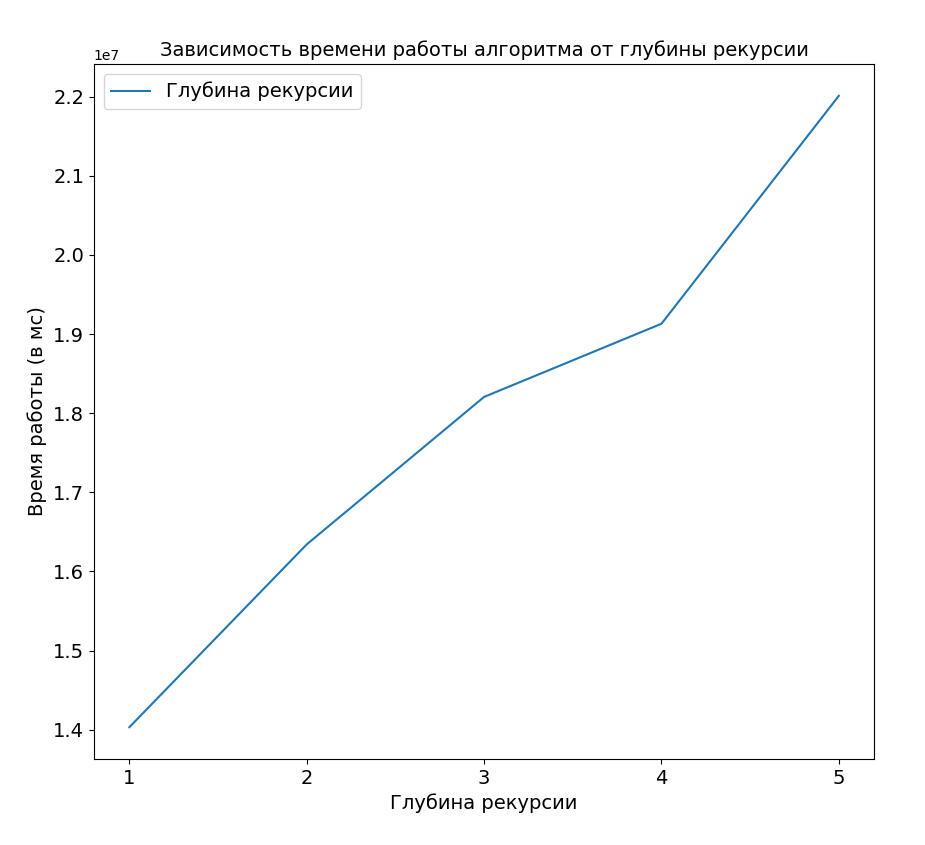
\includegraphics[width=\linewidth]{inc/recursion.png}
	\end{center}
	\caption{График зависимости времени работы алгоритма от глубины рекурсии}
\end{figure}
\FloatBarrier

\section{Выводы}
Время работы алгоритма обратной трассировки лучей зависит от его параметров и характеристик фигур, которые присутствуют в сцене.
Алгоритм работает при 4 фигурах на 30\% быстрее, если фигуры закрашиваются цветом, а не покрываются текстурами.
Быстрее всего обратная трассировка лучей работает при $N = 8$ потоках, что соответствует количеству ядер в системе.
Также выявлена прямая зависимость времени работы алгоритма от глубины рекурсии.